\apendice{Documentación de usuario}

\section{Introducción}

En este manual se detallan los requerimientos para utilizar todas las funcionalidades de PrimeBot y poder aprovechar cada uno de los parámetros que hay en la programación del robot.

\section{Requisitos de usuarios}

Los requisitos mínimos para poder utilizar el proyecto son:

\begin{itemize}
\tightlist
\item
  Disponer de un kit de PrimeBot con main.ino cargado
  \item
  Disponer de un móvil Android o un equipo con conexión Bluetooth
  \item
  Disponer de una aplicación como Monitor Serial
\end{itemize}

\section{Instalación}

Si el usuario ya dispone del programa main.ino cargado en la placa de Arduino correspondiente y una aplicación de monitor serial instalada en el dispositivo a conectar, no deberá realizar ninguna instalación adicional.

\section{Manual del usuario}

En esta sección se describe el uso de las diferentes funcionalidades de PrimeBot
\subsection {Conexión Bluetooth}

Antes de ejecutar cualquier programa, debemos encender PrimeBot y realizar la conexión Bluetooth.
Cuando esta conexión esté hecha, el LED rojo del módulo Bluetooth permanecerá fijo.

\subsection {Modo Calibración}

El modo calibración corresponde a la posición 0000 del dip switch que está integrado en la placa de control.

Cuando se quiere utilizar PrimeBot, este es el primer modo que debemos ejecutar ya que en este modo se realiza la calibración de los sensores siguelíneas QTR y se establece la conexión Bluetooth con el robot.
El orden correcto de ejecución será:

\begin{enumerate}
\def\labelenumi{\arabic{enumi}.}
\tightlist
\item
Seleccionamos la posición 0000 en el switch.
\item
Se pulsa el botón de selección de programa.
\item
Mientras la luz LED de la plaza arduino esté encendida de forma fija, debemos hacer pasadas suaves sobre la línea negra que debe seguir, de esta forma estaremos calibrando los sensores.
\item
Cuando acabe la calibración de los sensores, los motores se moverán durante un segundo indicando que la calibración ha terminado.
\item
Ahora podemos realizar la conexión Bluetooth con PrimeBot desde nuestro dispositivo.
\end{enumerate}

\begin{figure}[h]
	\centering
	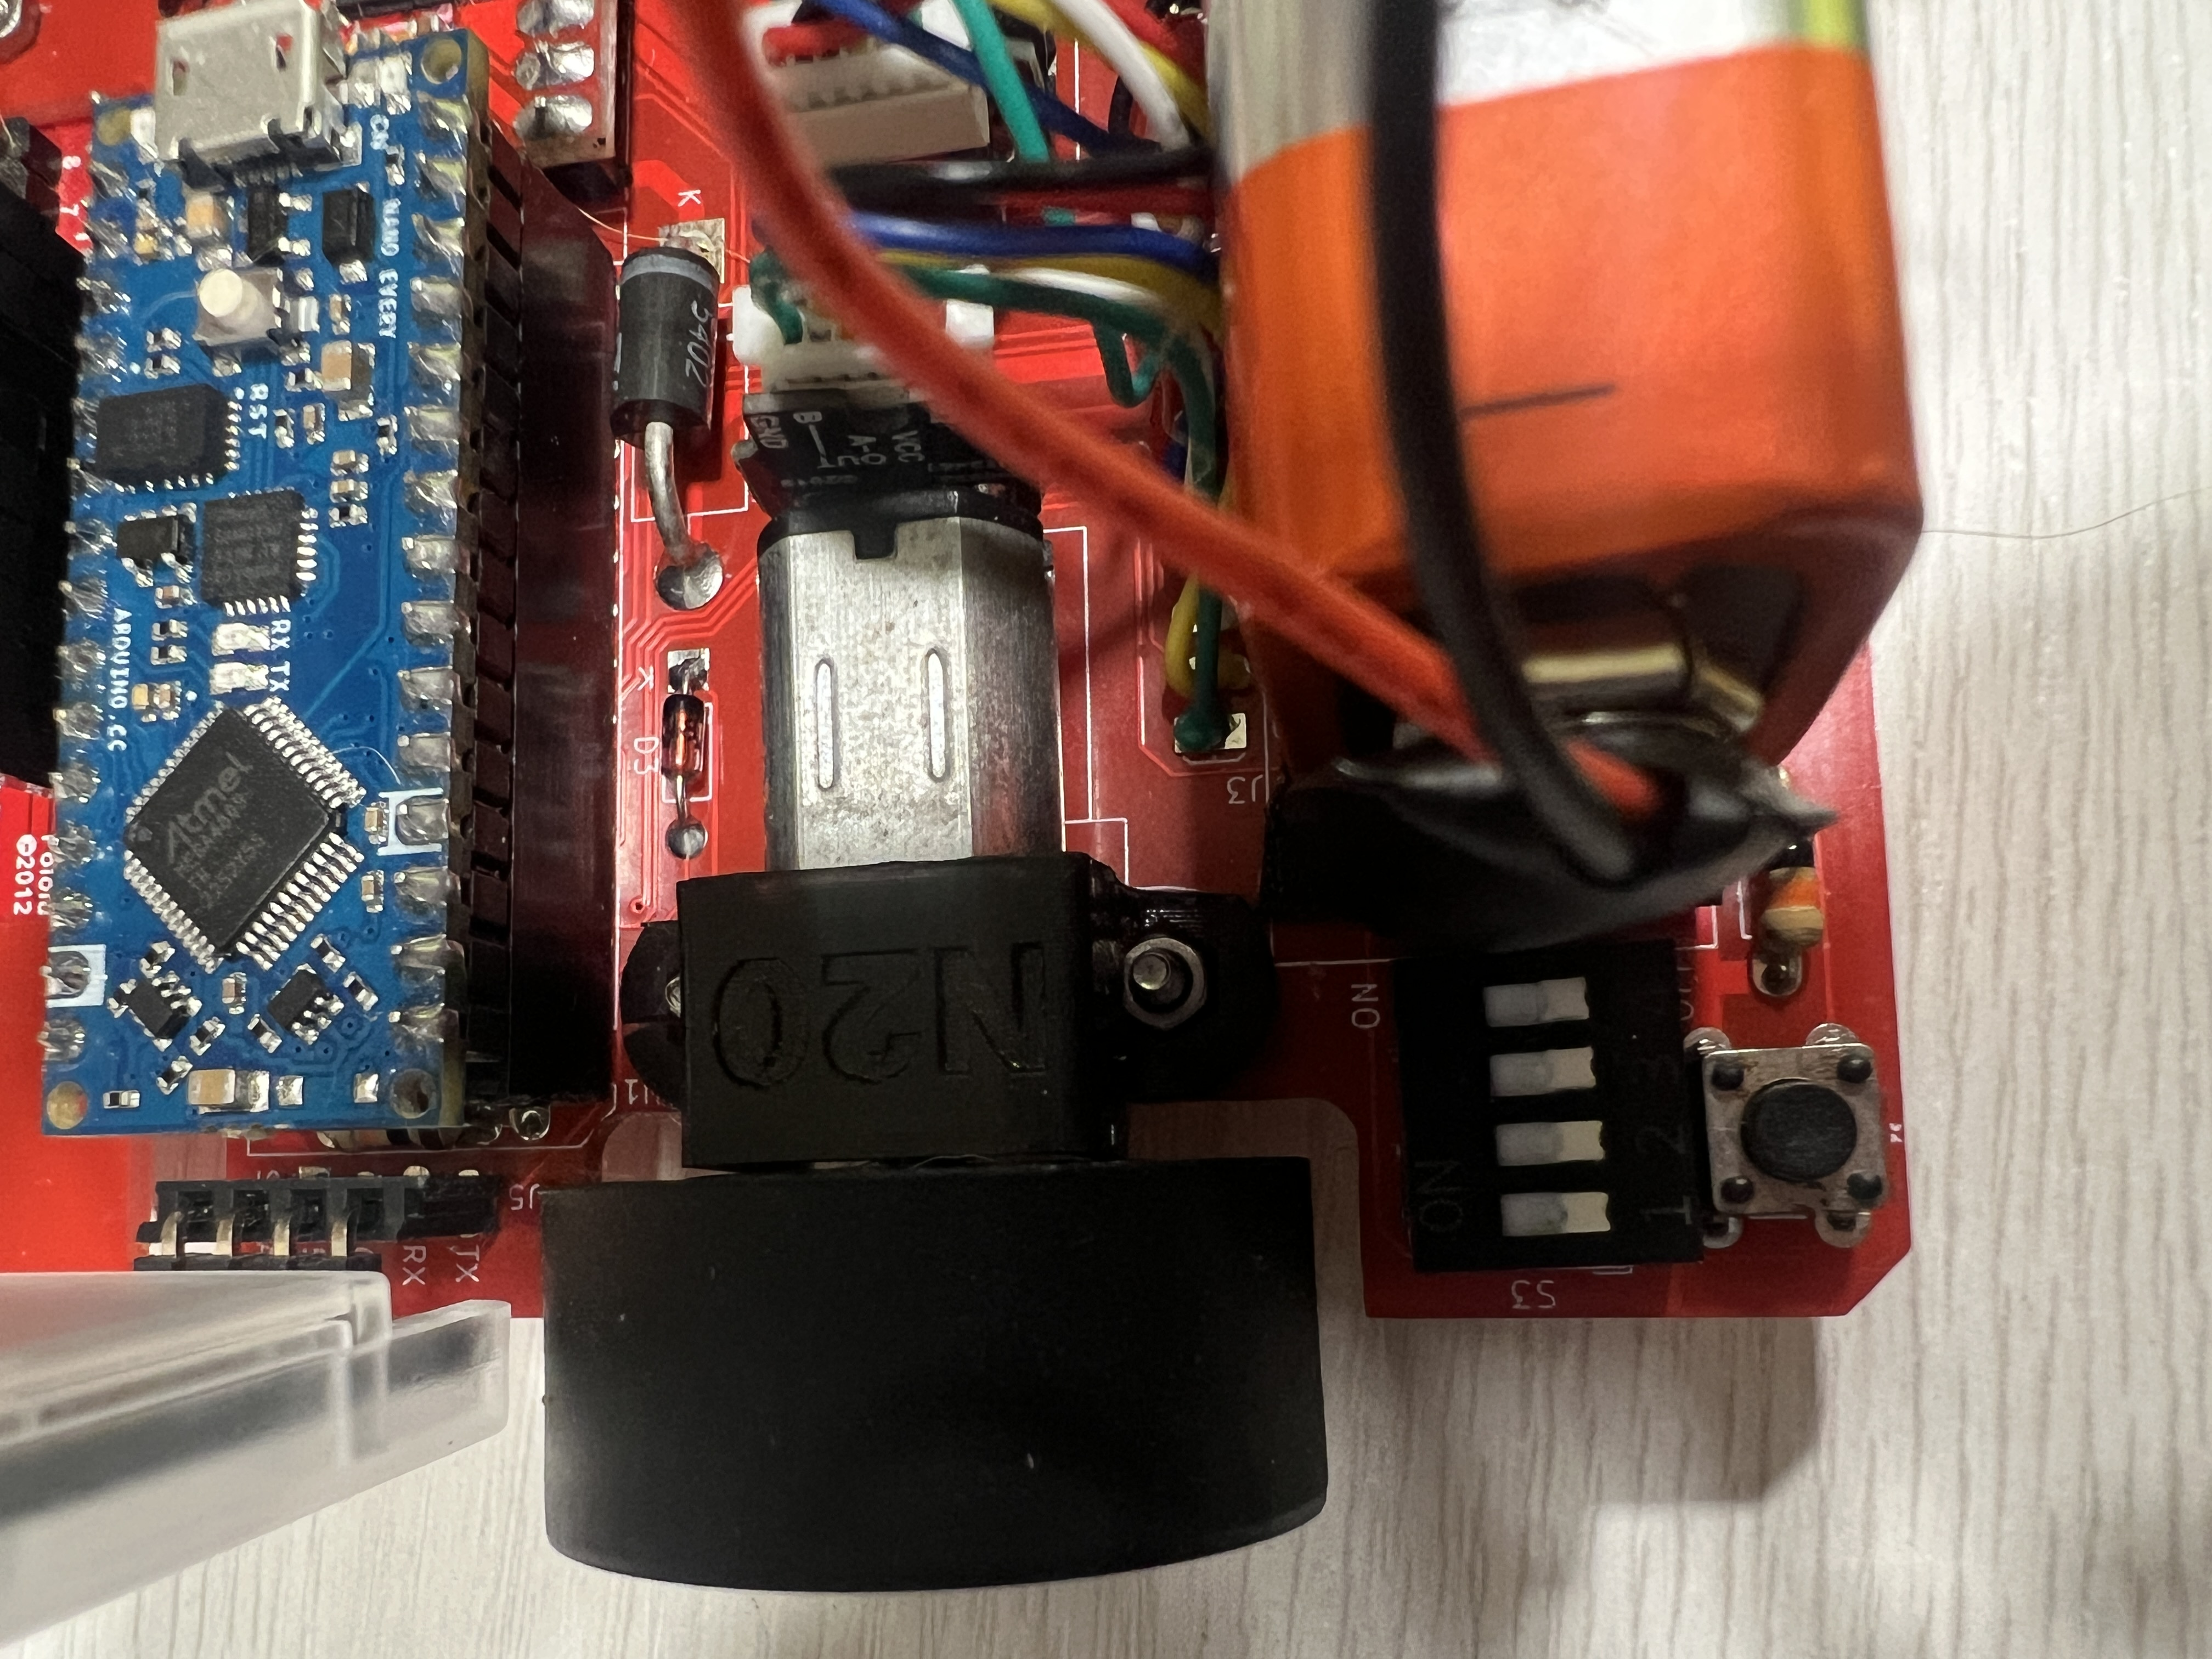
\includegraphics[width=0.5\textwidth]{anexos/0000}
	\caption{Posición Modo Calibración}
	\label{fig:E.1}
\end{figure}


\subsection {Modo Siguelíneas}
Esta funcionalidad corresponde a la posición 0001 del dip switch integrado en la placa de control.
El modo siguelíneas consiste en el seguimiento de una línea negra sobre un fondo blanco de cara a realizar las vueltas al circuito cerrado en el menor tiempo posible y con la mayor estabilidad posible del robot.

\begin{enumerate}
\def\labelenumi{\arabic{enumi}.}
\tightlist
\item
Tras realizar la calibración y la conexión por Bluetooth, colocaremos a PrimeBot sobre la línea negra a seguir.
\item
Colocaremos el switch en la posición 0001.
\item
Se pulsa el botón de selección de programa.
\item
Si hemos hecho bien los pasos en la aplicación de Monitor Serial veremos un mensaje indicando que se ejecutará el código correspondiente a la prueba siguelíneas.
\item
PrimeBot comenzará a moverse por la línea negra
\end{enumerate}

\begin{figure}[h]
	\centering
	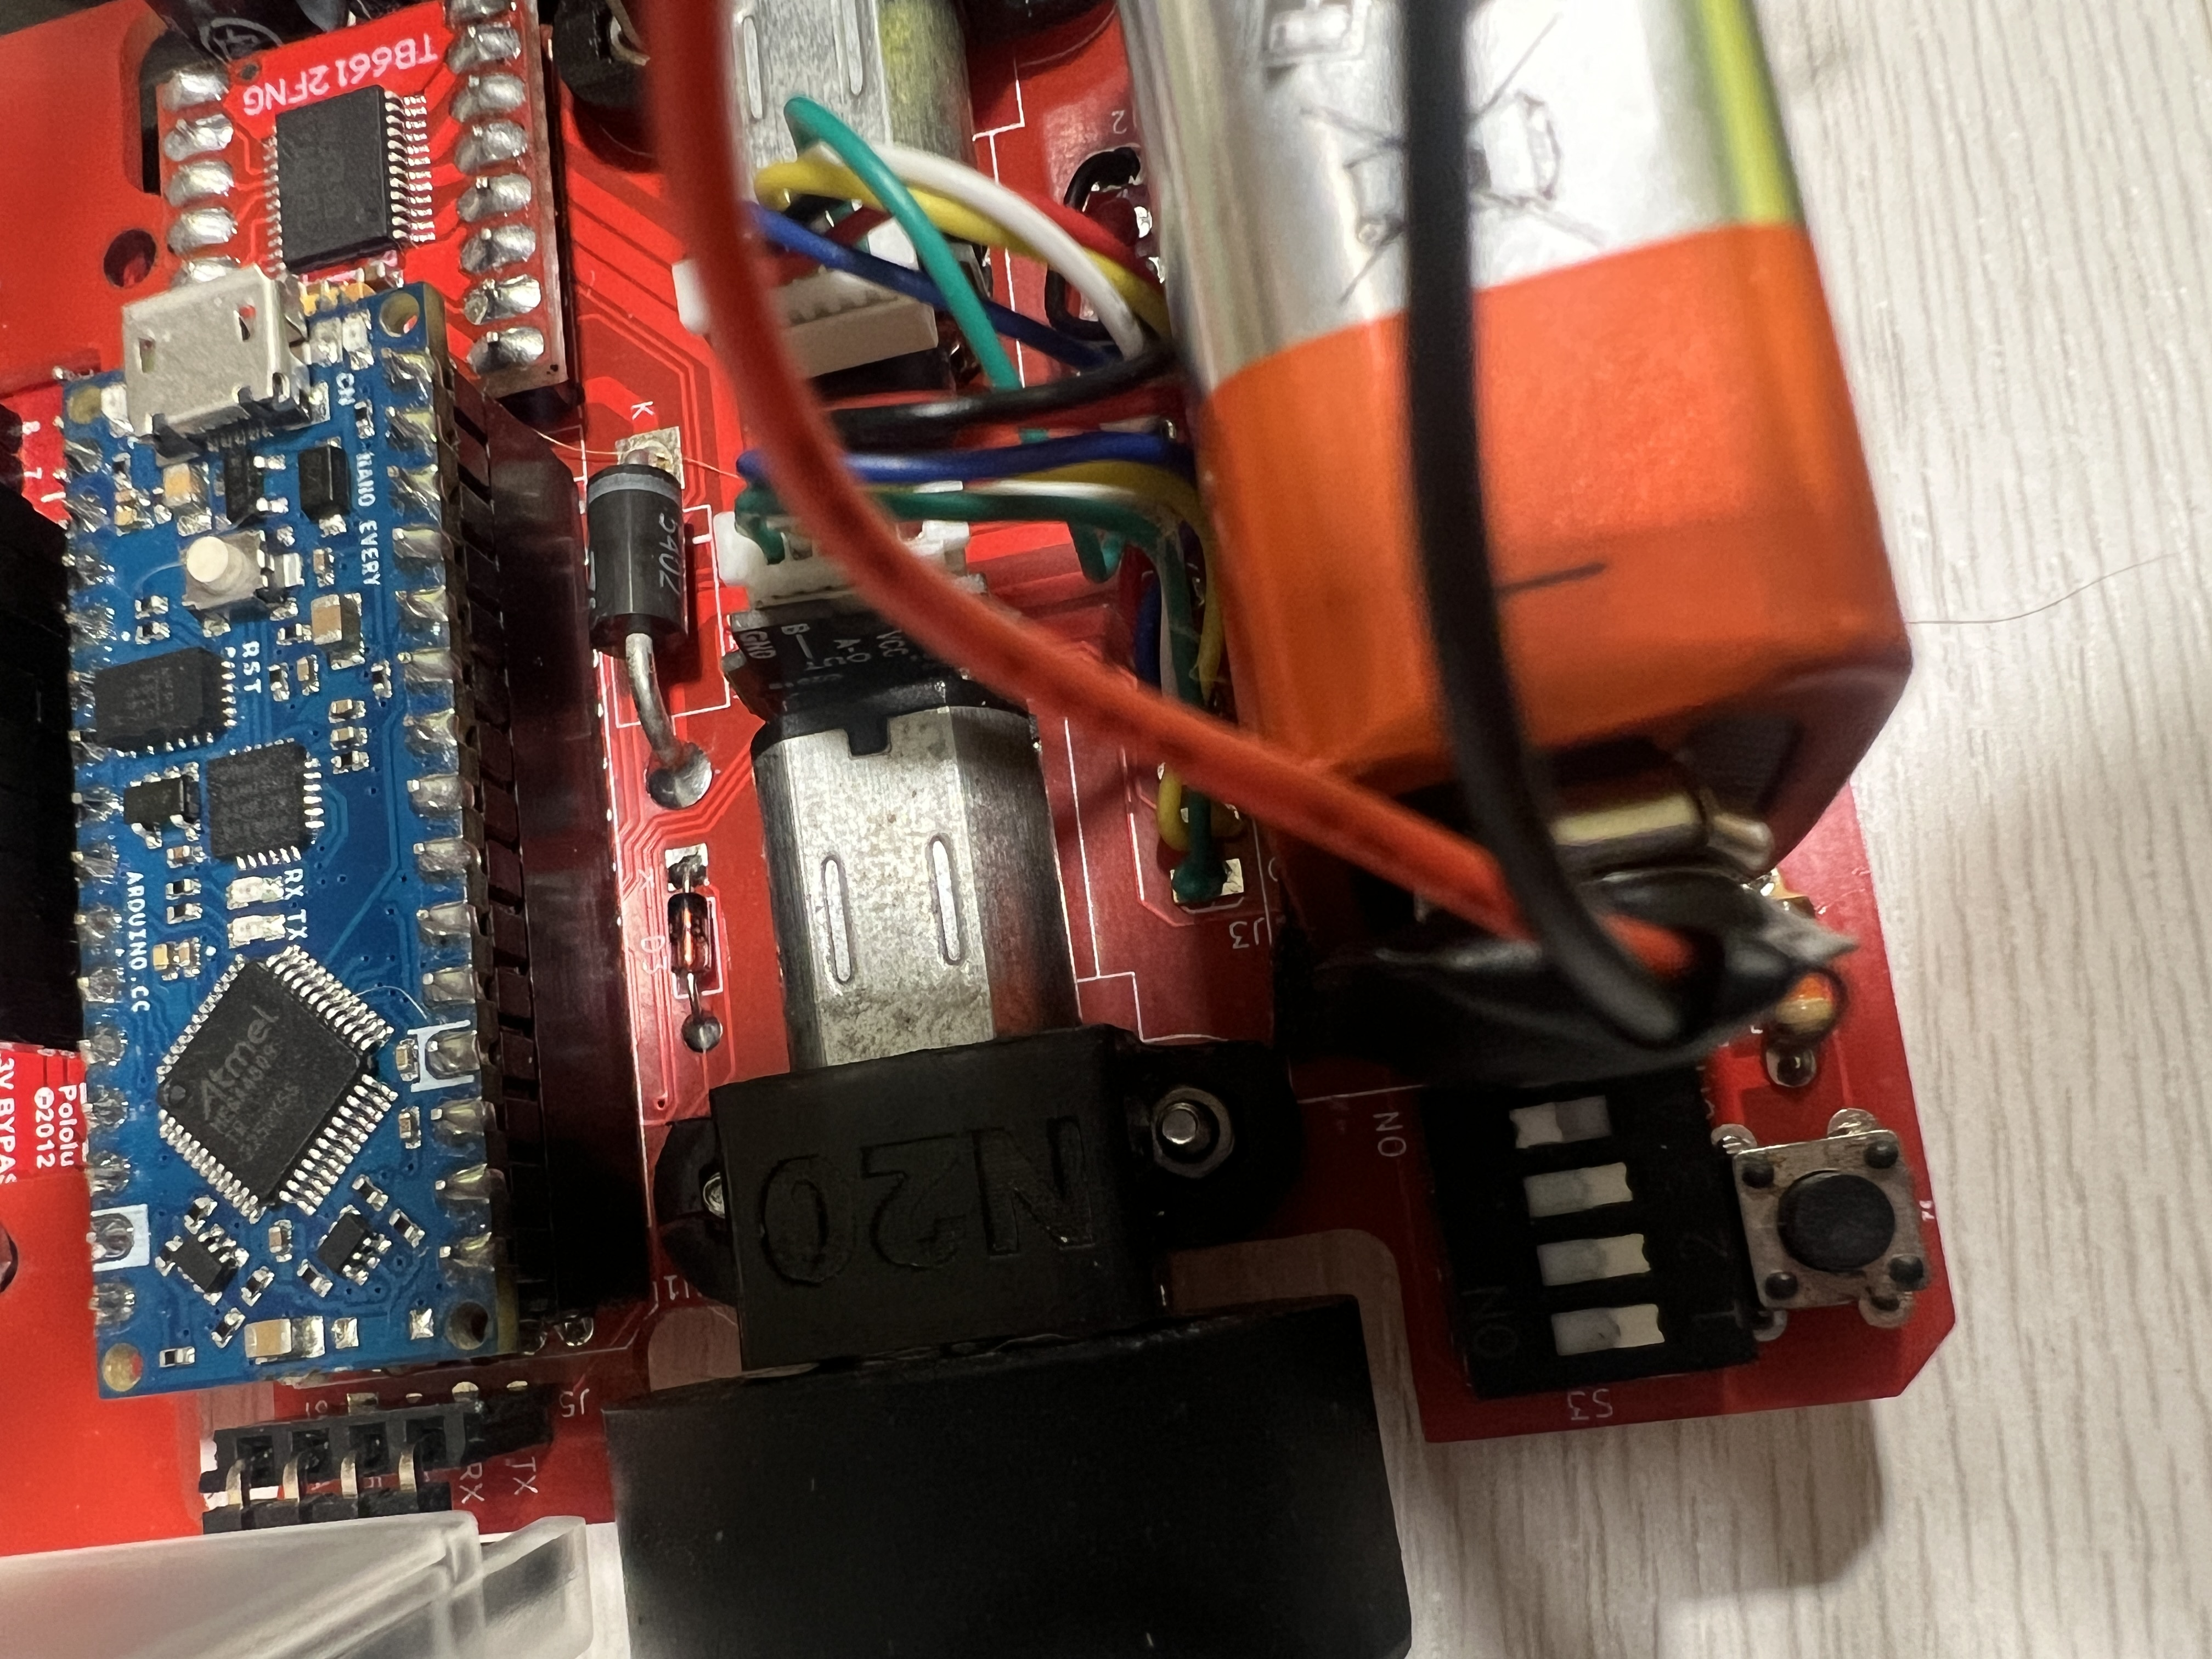
\includegraphics[width=0.5\textwidth]{anexos/0001}
	\caption{Posición Prueba Siguelíneas}
	\label{fig:E.1}
\end{figure}

A la vez que se está ejecutando este algoritmo y PrimeBot se va moviendo, en el Monitor Serial veremos impresos diferentes parámetros los cuales son configurables enviando carácteres a través de Monitor Serial de la siguiente forma:
\begin{itemize}
\tightlist
\item
  P: Aumentará la variable Kp en 0.1
  \item
  p: Reducirá la variable Kp en 0.1
  \item
  I: Aumentará la variable Ki en 0.01
   \item
  i: Reducirá la variable Ki en 0.01
   \item
  D: Aumentará la variable Kd en 0.1
   \item
  d: Reducirá la variable Kd en 0.1
   \item
  V: Aumentará la variable Kv en 0.01
   \item
  v: Reducirá la variable Kv en 0.01
   \item
  B: Aumentará la variable Velocidad base en 1
   \item
  b: Reducirá la variable Velocidad base en 1
\end{itemize}

\subsection {Modo Cuadrícula}
Esta funcionalidad corresponde a la posición 0010 del dip switch integrado en la placa de control.

El modo cuadrícula está pensado para la navegación de PrimeBot a través de una cuadrícula ya definida en dimensiones y otorgando a PrimeBot una estación de origen y una de destino.
La ejecución correcta de este programa será:

\begin{enumerate}
\def\labelenumi{\arabic{enumi}.}
\tightlist
\item
Seleccionamos la posición 0010 en el switch.
\item
Se pulsa el botón de selección de programa.
\item
Colocamos a PrimeBot en la estación de origen que corresponda.
\item
A través del monitor serial nos comunicaremos con PrimeBot.
\item
El primer parámetro que tenemos que poner es el número de puntos bloqueados, en caso de poner un valor mayor que 0, PrimeBot solicitará las coordenadas X e Y de los puntos bloqueados.
\item
Seguido nos solicitará la estación de Origen donde ya está situado PrimeBot.
\item
Por último nos solicitará la estación de destino.
\item
PrimeBot comenzará a navegar por la cuadrícula hasta llegar a la estación de destino.
\end{enumerate}

\begin{figure}[h]
	\centering
	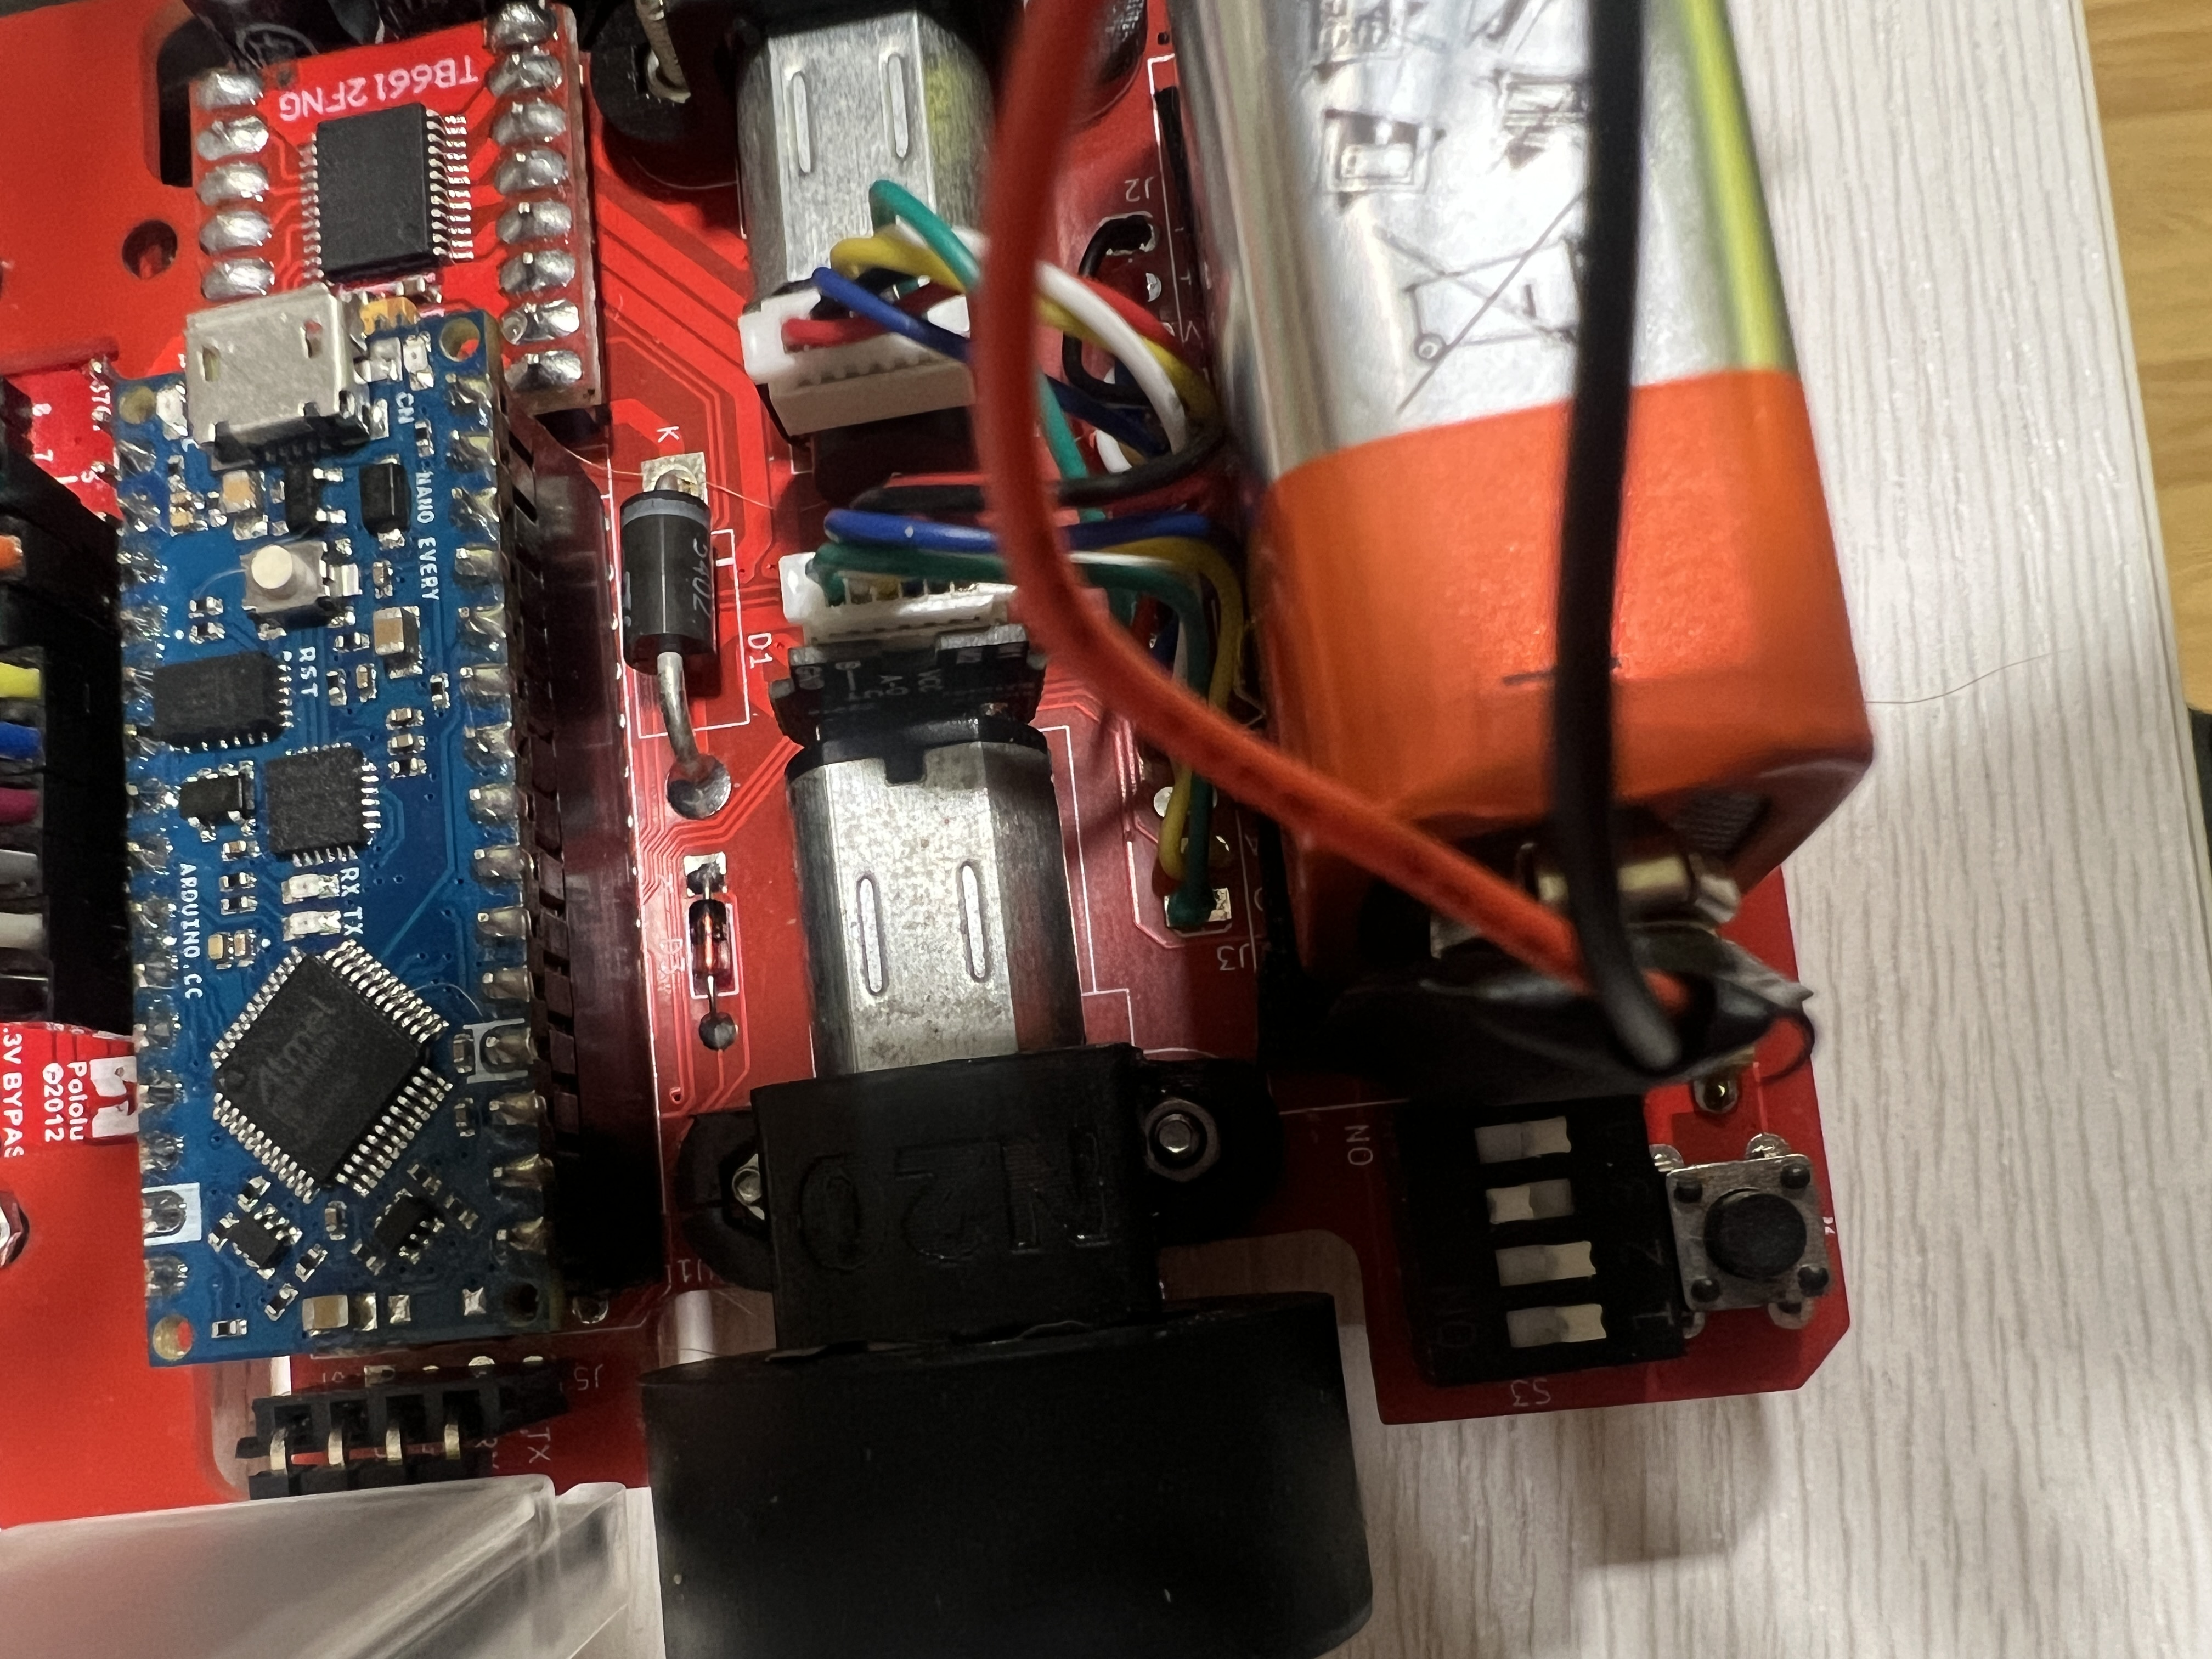
\includegraphics[width=0.5\textwidth]{anexos/0010}
	\caption{Posición Prueba Cuadrícula}
	\label{fig:E.1}
\end{figure}

En el caso de que no sea posible calcular una ruta debido a los puntos bloqueados, PrimeBot nos lo comunicará por el Monitor serial y se deberá pulsar de nuevo el botón de selección de programa.
Además, a través del monitor serial PrimeBot imprimirá una cuadrícula igual a la real indicando tanto el recorrido que está realizando como los puntos bloqueados.

Esta prueba también emplea un algoritmo PID para navegar a través de la cuadrícula por tanto podemos modificar los parámetros que hemos nombrado en el apartado anterior si lo vemos necesario.

\subsection {Modo Laberinto}
Esta funcionalidad corresponde a la posición 0011 del dip switch integrado en la placa de control.
\begin{enumerate}
\def\labelenumi{\arabic{enumi}.}
\tightlist
\item
Seleccionamos la posición 0011 en el switch.
\item
Colocamos a PrimeBot en el origen del laberinto.
\item
PrimeBot recorrerá el laberinto hasta encontrar la salida.
\end{enumerate}

\begin{figure}[h]
	\centering
	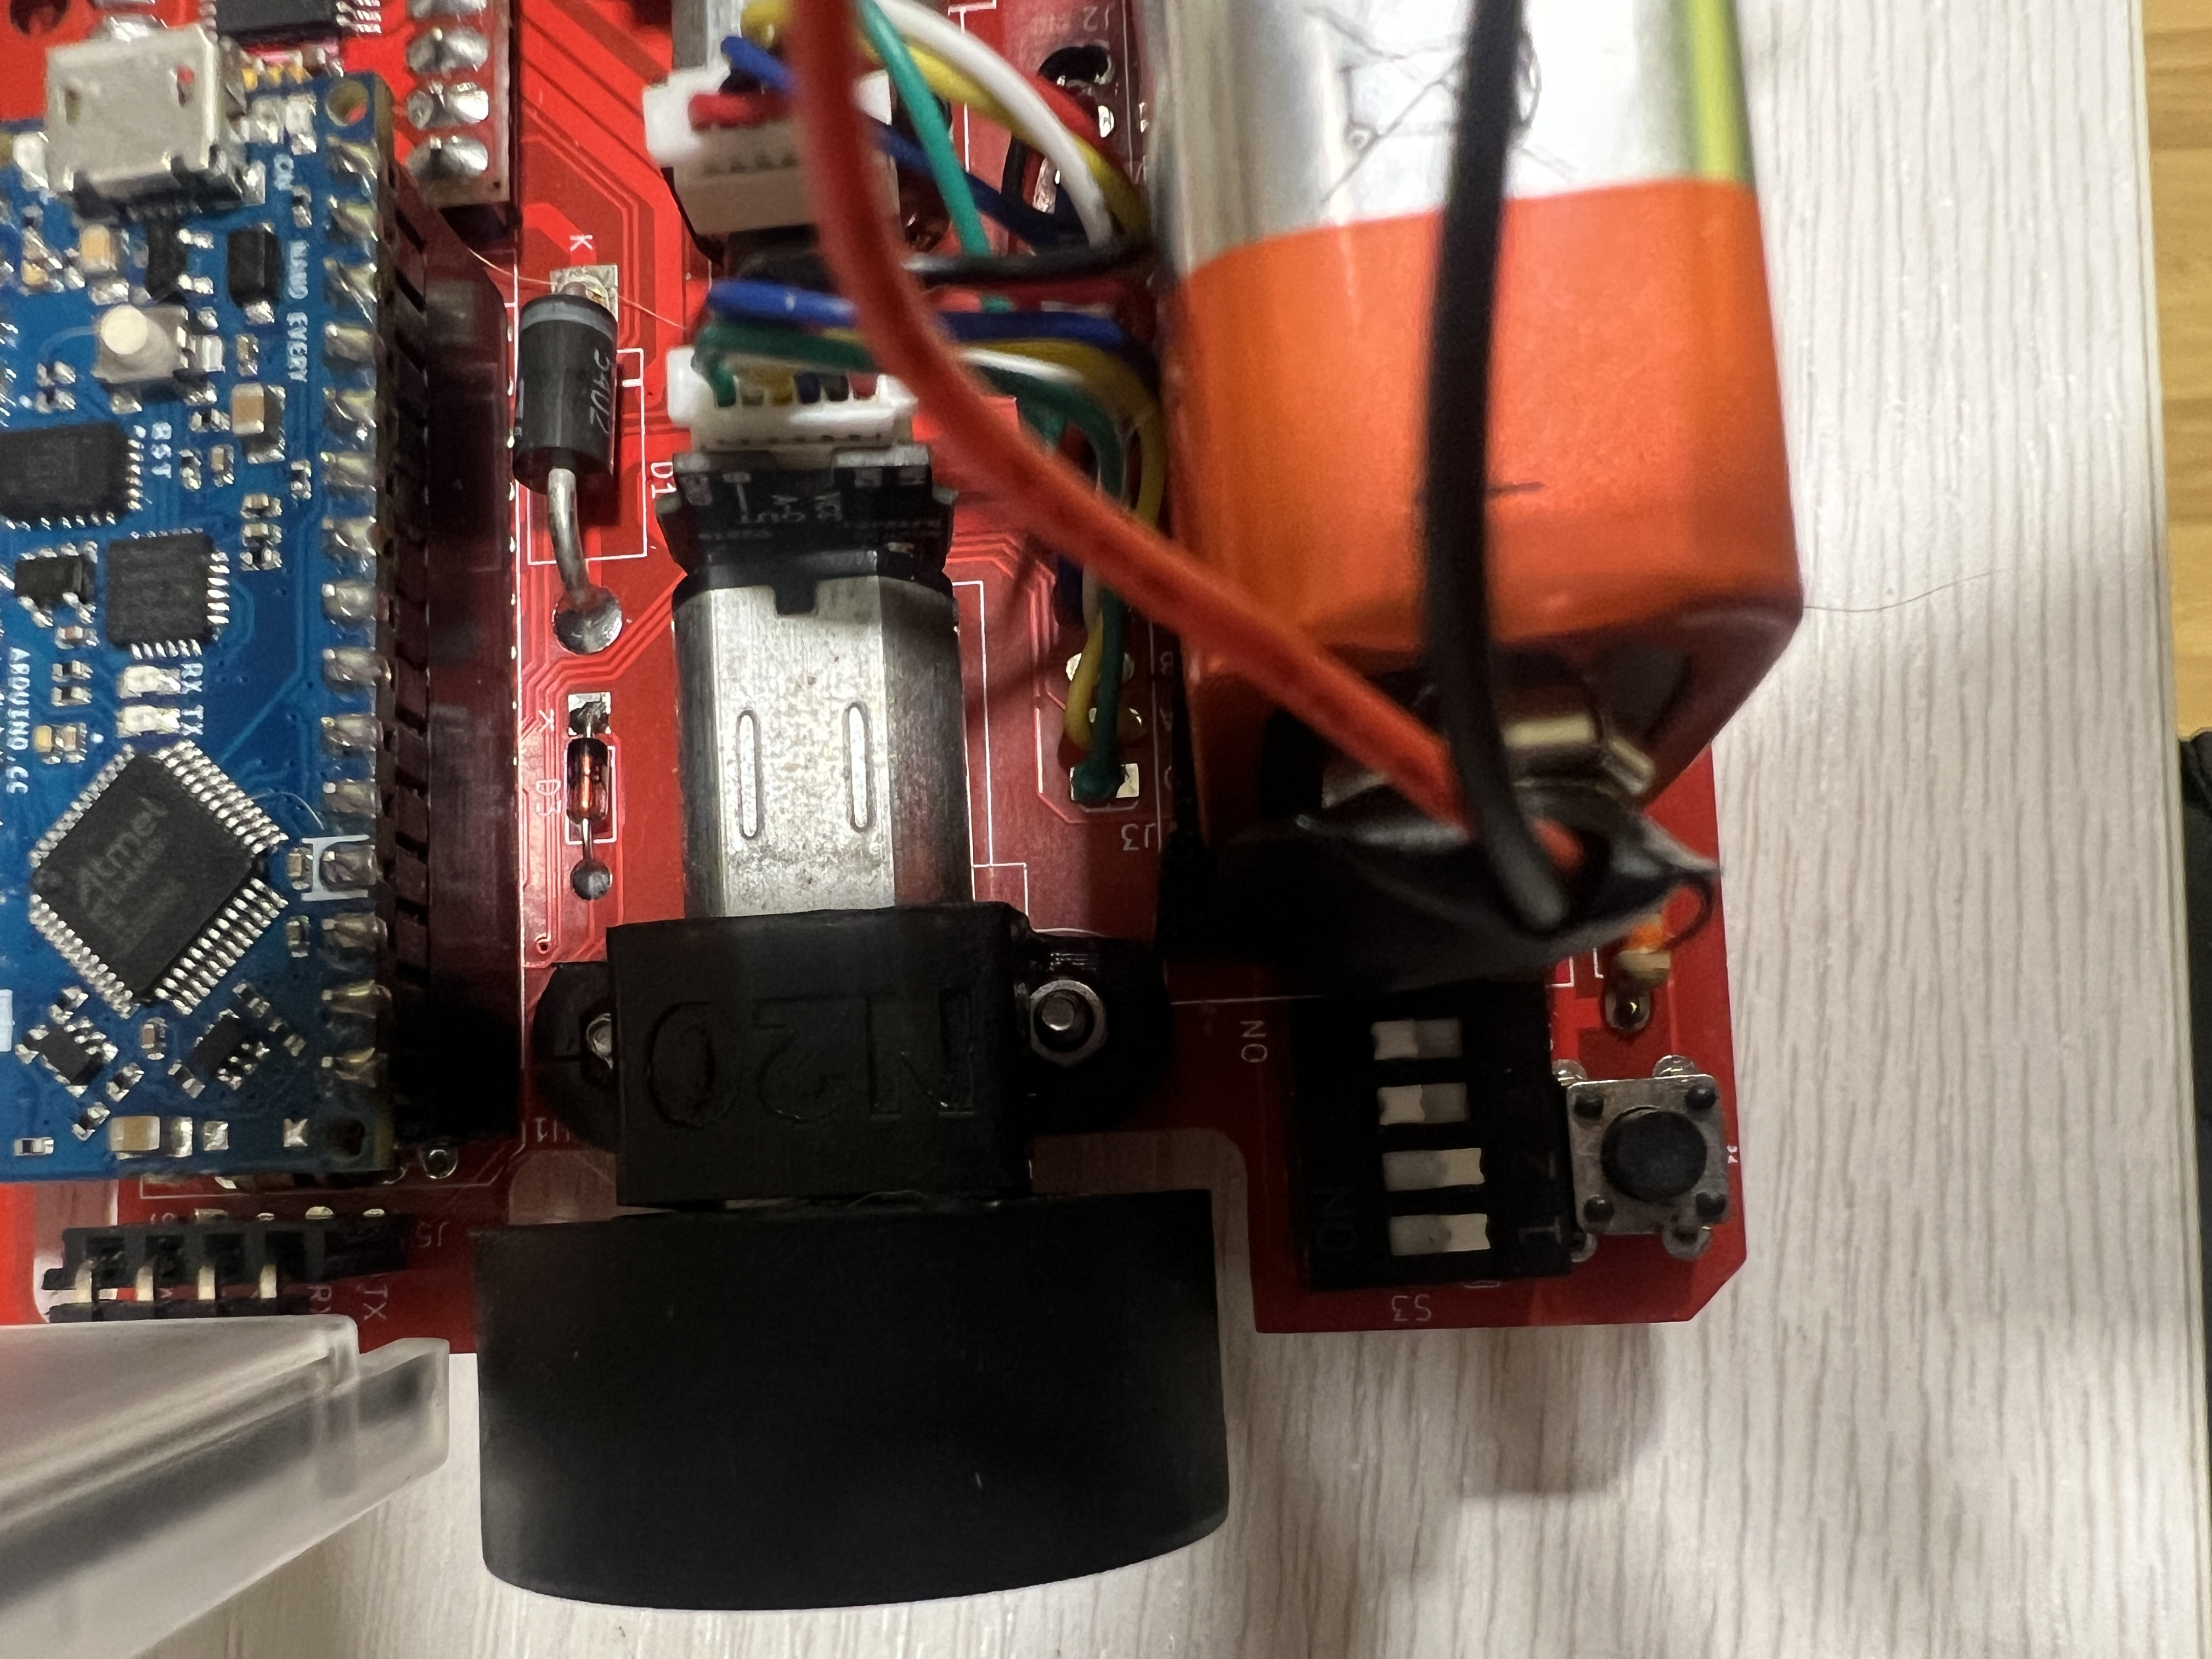
\includegraphics[width=0.5\textwidth]{anexos/0011}
	\caption{Posición Prueba Laberinto}
	\label{fig:E.1}
\end{figure}
